\chapter{Sharemind: A Secure Computing Platform}\label{c:sharemind}

Sharemind \cite{bogdanov2008sharemind, bogdanov2013sharemind} is a general purpose SMPC system, for privacy preserving data processing operating on additively secret-shared values.
The idea of Sharemind is to provide a secure infrastructure that is able to host and evaluate privacy preserving algorithms.
Sharemind provides an easily programmable and flexible platform that enables non\hyp cryptographers to develop and test privacy preserving algorithms such as Privacy Preserving Data Mining (PPDM).
It consists of the computation runtime environment and a programming library for creating private data processing applications
Sharemind is provably secure under the semi-honest (honest but curious) setting.

Sharemind’s is deployed as a distributed computation platform, that can be used both for data storage and computation.
The deployment model consists of (usually three) nodes, the computing nodes that use SMPC through secret sharing to privately process the data.
Secret sharing guarantees data confidentiality during storage.
All computations are done by the dedicated computing nodes.

Data providers submit their private inputs by sending the corresponding cryptographic shares to the computing nodes.
The secret sharing scheme ensures that each share is a random bit string.
Each host, computing node, is not able to decrypt the data, or even extract any information about them.
Consequently, a node holding that share learns no extra information about the data input (secret), than if they did not hold that share.
For that reason, data providers need not trust any of the computing nodes.
Instead providers must trust that the nodes as a group obey a set of rules such as that they do not collude during the computations.
This can be achieved through physical and organizational security measures as well as software auditing.
In practice, the computing nodes will be servers run by independent entities, such as companies or government agencies, ideally having conflicting interests.
Data users want to analyze the information given by data providers.
Answers to their queries are given through the Sharemind system, and not from data providers directly.


The Sharemind framework provides a privacy preserving  instruction set which includes secure addition, multiplication and greater\hyp than\hyp or\hyp equal comparison of two shared values.
Multiplication of a shared value with a constant and extraction of its bits as shares is also possible.
Bit extraction and arithmetic primitives are sufficient to construct any Boolean circuit with a linear overhead and thus the Sharemind framework is also Turing complete \cite{bogdanov2008sharemind}.
Many data mining and statistical analysis algorithms use no other mathematical operations than the Sharemind's instruction set, thus it is sufficient for most applications.




\section{Real World Applications}\label{s:real-world-applications}

\subsection{Satellite Collision Detection}\label{s:satellite-collision-detection}
One notable example of a real world application of SMPC using Sharemind was presented in \cite{kamm2015secure}.
In this paper, Sharemind engine was utilized to perform satellite collision detection in a secure multiparty setting.
The number of satellites orbiting our planet is growing, and so does the danger of collisions.
Indeed, two satellites crashed in 2009.
Satellite owners, such as governments, do not want to reveal orbital information about their satellites.
However, satellites come with extravagant expenses and each satellite owner want to protect their property.

Future collisions could be avoided by sharing information about the satellites orbits.
Using SMPC, the parties can cooperate and learn whether a collision is going to happen and nothing else.
No information about the actual orbits would leak -- no party can see the individual values, since computations are carried out on encrypted data.
The SMPC solution provides cryptographic guarantees for the confidentiality of the input trajectories.


\subsection{Analysing Private Databases}\label{s:analysing-private-databases}
Another worth mentioning application took place in 2015, where the Estonian Center of Applied Research used Sharemind to collect governmental tax and education records with purpose to run a big data study looking for correlations between people who work during their studies and those who fail to graduate in time.

In Estonia -- where this research took place, the Ministry of Education and Science keeps track of students and the Tax and Customs Board keeps track of working (by tracking income tax payments).
A correlation between working during studies and not graduating in time could be possible to find, if these databases were not private.
However, this data cannot be shared because of the Personal Data Protection Act and the Taxation Act and also many European Union regulations, such as General Data Protection Regulation (GDPR) \cite{gdpr}.
All these legislation prevents such studies from being performed.

The results of the study were quite surprising.
The study found no relation between working during studies and not graduating on time.
Instead, it turned out that the population group that was studied (Estonian students of all fields) work an equal amount.
Moreover, it showed an obvious the reduction of employment during the financial crisis in 2008.
This study would not have been possible without an SMPC engine such as Sharemind, as no research organization can gain access to these private databases due to Data Protection regulations.
Nevertheless, this research allowed more personalized follow-up studies to be planned for finding the reasons why students quit.



\section{SecreC}\label{s:secrec}

The programmer of the privacy preserving applications does not necessarily know the underlying security protocols.
Application are developed using the SecreC programming language \cite{jagomagis2010secrec}.
SecreC is an procedural imperative domain specific language (DSL) that is syntactically similar to C. SecreC guarantees writing privacy-preserving algorithms without any knowledge of the underlying cryptographic protocol.
In other words, SecreC distinguishes the application\myslash business logic from the cryptographic protocol.

The language uses a custom type system, which separates private\myslash confidential data from public.
Public values are processed as usual, whereas private values, which are in secret-shared form are processed using secure computation.
To achieve this, SecreC adds a security type to each fundamental data type.
The security type can be either \textit{private} or \textit{public}.
If no security type is specified then the public one is used by default.
Security types differ from standard data types in the sense that data associated with the public security type will be stored and processed publicly on the Sharemind virtual machine, whereas data associated with the private security type, will be stored in secret\hyp shared form.
Each computing node will acquire one share of the actual value.

In SecreC one can have expressions of private or public data.
In the case that such two expressions are combined into a single expression, the public data are secret\hyp shared and moved into the private execution environment in order for the composite expression to be evaluated.
That way all data are of the private security type and the expression can be evaluated.

Sometimes however it is vital to open a secret.
This could be done in order to gain some insight about an algorithm having good intentions in mind.
SecreC offers a special \f{Declassify} operator through which is made possible to publish private information.
An expression that is declassified has its security type changed from private to public, and the secret\hyp shared value moves into the public execution environment.
Since the use of the \f{Declassify} operator is the only way for private data to become public, its use should be tracked in order to reason about data privacy and to avoid potential unwanted privacy leaks.
As a rule of thumb, declassification of private data should occur ass little as possible.
Ideally, declassification should be used only to publish the final results of an algorithm, or intermediate results that have low privacy risk \textit{i.e.} do not reveal sensitive information.

Typically, if a decision (\textit{e.g.} a branch) is to be made over private data, that would require the data to be published, that is to be converted to the public security type.
For instance, consider the following example:

\texttt{if (x) a = b; else a = c; }

One can rewrite the previous statement using with the following expression:

\texttt{a = b * x + c * (1-x); }

Using this technique a programmer can replace conditional statements on private data with such oblivious selection clauses.
So the control flow dependencies are converted into data dependencies.

{
\begin{minted}[xleftmargin=21pt, framesep=3mm, frame=single, linenos, tabsize=2, breaklines, breaksymbolleft=, fontsize=\footnotesize]{c++}
pd_shared3p uint64 max(pd_shared3p uint64 x, pd_shared3p uint64 y) {
  pd_shared3p uint64 gt = (uint64)(x > y); // 1 if x > y, 0 otherwise
  return x * gt + y * (1-gt); // Oblivious selection of the max value
}

void main(){
  pd_shared3p uint64 x1 = 5; // Private, secret-shared value of input party 1
  pd_shared3p uint64 x2 = 8; // Private, secret-shared value of input party 2
  pd_shared3p uint64 max = max(x1, x2); // Private result
  print(declassify(max)); // Result publishing
}
\end{minted}
\captionof{lstlisting}{Millionaire problem in SecreC}\label{l:millionaires}
}

An example of SecreC code can be found in Code Snippet \ref{l:millionaires}.
The problem at hand is Yao's millionaire problem \cite{yao1982protocols} as described in section \ref{s:smpc}.
Here we use \texttt{pd\_shared3p} as the security type, which stands for \textit{\textbf{p}rotection \textbf{d}omain \textbf{shared 3 p}arties}, and corresponds to a private security type using secret\hyp sharing between three parties.


\subsection{SIMD in SecreC}\label{ss:simd-secrec}

Each SMPC operation in Sharemind is implemented as an assembly instruction.
Sharemind also supports vectorized operations which play a significant role in the program's efficiency.
With vectorized operations the same protocol is executed but using multiple inputs at once, in parallel.
Using such SIMD (Single Input Multiple Data) instructions the protocol performs all operations in parallel by packaging the values in a single communication message.

This significantly reduces the communication overhead between the participating parties, which is usually a dominating factor in a protocol's performance.
Thus, developing applications with vectorization in mind, has a substantial contribution to the application's efficiency.
We have focused on using vectorization as much as possible when developing our privacy preserving algorithms, which we describe in chapter \ref{c:pp-algorithms}.

Below, in code snippets \ref{l:non_vectorized_addition} and \ref{l:vectorized_addition}, we present two versions of array addition in SecreC.
The first one works with a typical loop on each of the array elements, while the second one works by performing an SIMD addition between two arrays.

{
\begin{minted}[xleftmargin=21pt, framesep=3mm, frame=single, linenos, tabsize=2, breaklines, breaksymbolleft=, fontsize=\footnotesize]{c++}
  void main(){
    uint64 N = 5;
    pd_shared3p uint64 a(N) = {1, 2, 3, 4, 5}; // Array definition of size N
    pd_shared3p uint64 b(N) = {6, 7, 8, 9, 10}; // Array definition of size N
    pd_shared3p uint64 c(N); // Array declaration of size N
    for (uint64 i = 0; i < N; i++){
      c[i] = a[i] + b[i]; // Element-wise addition with sequential access
    }
    print(declassify(c)); // Result publishing
  }
\end{minted}
\captionof{lstlisting}{Array addition in SecreC}\label{l:non_vectorized_addition}
}

{
\begin{minted}[xleftmargin=21pt, framesep=3mm, frame=single, linenos, tabsize=2, breaklines, breaksymbolleft=, fontsize=\footnotesize]{c++}
  void main(){
    uint64 N = 5;
    pd_shared3p uint64 a(N) = {1, 2, 3, 4, 5}; // Array definition of size N
    pd_shared3p uint64 b(N) = {6, 7, 8, 9, 10}; // Array definition of size N
    pd_shared3p uint64 c(N) = a + b; // SIMD instruction of addition of the two arrays
    print(declassify(c)); // Result publishing
  }
\end{minted}
\captionof{lstlisting}{Array addition in SecreC using SIMD}\label{l:vectorized_addition}
}

The two example programs will have the same output but their performance will differ.
The first program will perform $N$ message exchanges between the computing parties for the addition, while the second will perform just one.
For large enough values of $N$, the performance difference is tremendous.



\section{Sharemind Infrastructure}\label{sharemind-infrastructure}
Sharemind consists of three different kinds of parties, input parties, computing parties and result parties.
The number of the input parties -- data providers -- as well as the result parties -- analysts/users -- is not restricted, however the computing parties are restricted by the SMPC protocol that is been used; for instance the aforementioned ``Millionaire problem" shown in (\textit{Source Code} \ref{l:millionaires}) uses the \textit{pd\_shared3p} security protocol, which utilizes three nodes.

As stated by Sharemind's author in \cite{bogdanov2013sharemind} three is usually the optimal number for the computing nodes configuration in the passively corrupted parties threat model.
Three is the lowest number for which an honest majority of parties processing secret shared data can be formed.
The number of parties can be less -- just two nodes -- but it adds more complexity to the protocols, as it requires more expensive cryptographic primitives to be used.
The number of computing parties can also be grater than three, increasing however the communication complexity.

An input party can also be the result party, or one of the computing nodes.
The data providers use secret sharing to distribute their confidential data between the computing nodes.
The analysts make queries and initiate computations, that are performed by the computing nodes leveraging the homomorphic primitives of the secret shares.
Finally, the analysts get the results of the private computation without anyone seeing the original confidential data.
Sharemind's infrastructure as explained in \cite{turban2014secure}, is presented in figure \ref{f:sharemind} in more detail.


\begin{figure}[th]
  \centering
  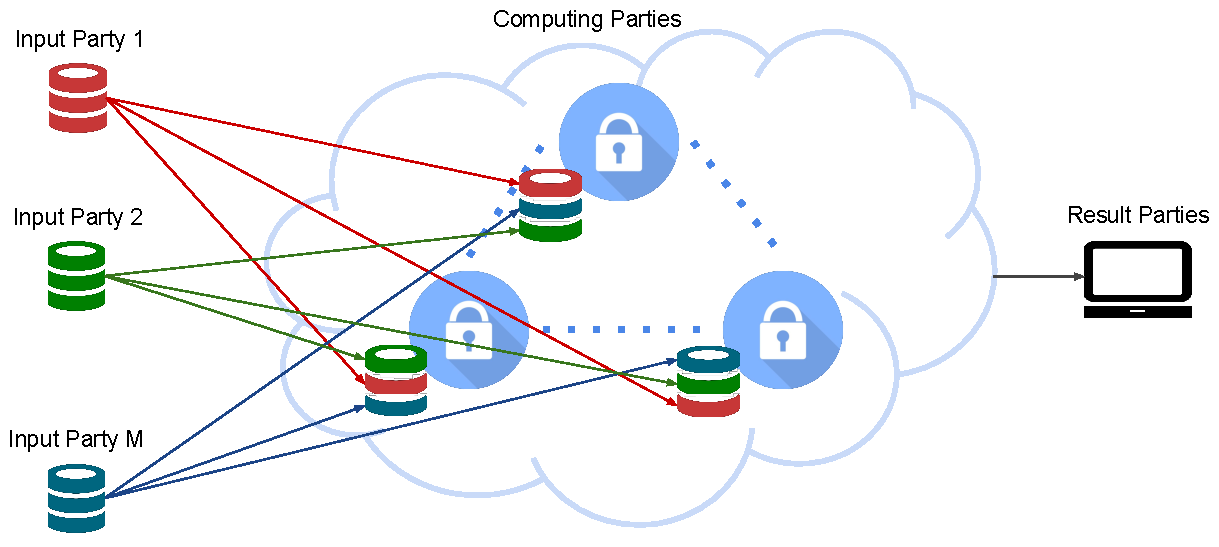
\includegraphics[width=\linewidth]{figures/sharemind_infrastructure.pdf}
  \caption{An overview of the architecture of Sharemind}\label{f:sharemind}
\end{figure}


